\documentclass[tikz,border=10pt]{standalone}
\usepackage{tikz}
\usetikzlibrary{positioning, fit, shapes.geometric, arrows.meta}

\begin{document}

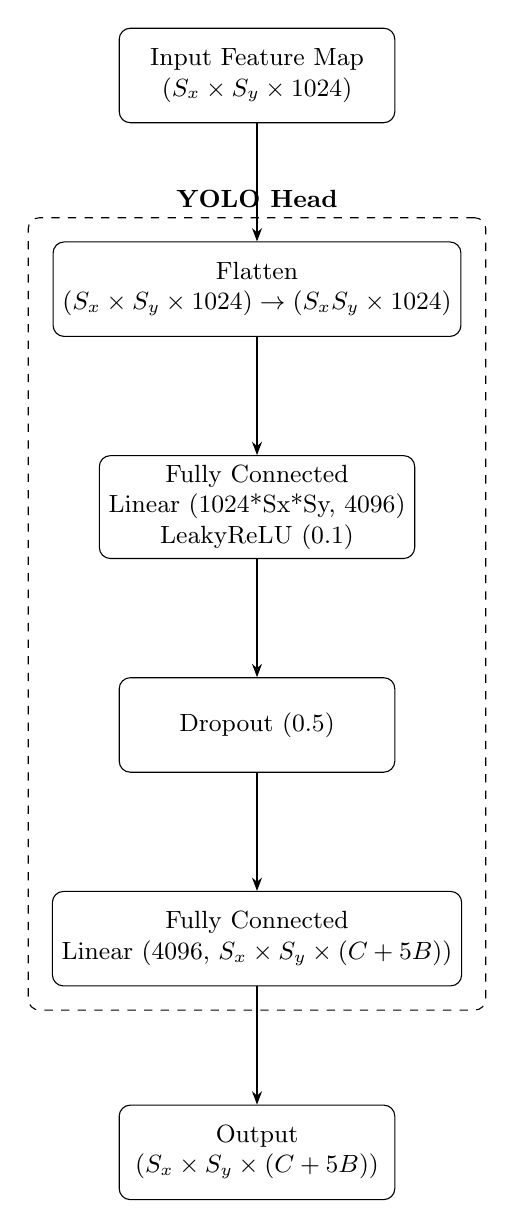
\begin{tikzpicture}[
    font=\small, 
    node distance=1.5cm, 
    >=Stealth, 
    block/.style={draw, rectangle, rounded corners, align=center, minimum width=3.5cm, minimum height=1.2cm},
    bigblock/.style={draw, dashed, rounded corners, inner sep=0.3cm}
]

% 输入特征图
\node[block] (input) {Input Feature Map\\\((S_x \times S_y \times 1024)\)};

% Flatten
\node[block, below=1.5cm of input] (flatten) {Flatten\\\((S_x \times S_y \times 1024) \to (S_x S_y \times 1024)\)};

% 全连接层1
\node[block, below=1.5cm of flatten] (fc1) {Fully Connected\\Linear (1024*Sx*Sy, 4096)\\LeakyReLU (0.1)};

% Dropout 层
\node[block, below=1.5cm of fc1] (dropout) {Dropout (0.5)};

% 全连接层2(最终输出)
\node[block, below=1.5cm of dropout] (fc2) {Fully Connected\\Linear (4096, \(S_x \times S_y \times (C + 5B)\))};

% 输出
\node[block, below=1.5cm of fc2] (output) {Output\\\((S_x \times S_y \times (C + 5B))\)};

% 连接箭头
\draw[->] (input.south) -- (flatten.north);
\draw[->] (flatten.south) -- (fc1.north);
\draw[->] (fc1.south) -- (dropout.north);
\draw[->] (dropout.south) -- (fc2.north);
\draw[->] (fc2.south) -- (output.north);

% 用虚线框标注 YOLO Head
\node[bigblock, fit=(flatten)(fc1)(dropout)(fc2), label=above:\textbf{YOLO Head}] (yolo_head) {};

\end{tikzpicture}

\end{document}
